\documentclass[12pt, letterpaper]{article}
\usepackage{amsmath}
\usepackage{amssymb}
\usepackage{latexsym}
\usepackage[usenames,dvipsnames]{xcolor}
\usepackage{graphicx}
\usepackage[headheight=15pt, margin=2.5cm]{geometry}
\usepackage{setspace}
\usepackage{longtable}
\usepackage{pdflscape}
\usepackage{ctable}
\usepackage{booktabs}
\usepackage{caption}
\usepackage{subcaption}
\usepackage[binary-units=true]{siunitx}
\usepackage{enumitem}
\usepackage{multirow}
\usepackage{float}
\usepackage{hhline}
\usepackage{tabulary}
\usepackage[nottoc, notlof, notlot]{tocbibind}
\usepackage[framed]{mcode}
%\usepackage{indentfirst}
\usepackage{standalone}
\usepackage{fancyhdr}
\usepackage{array}
\newcolumntype{P}[1]{>{\raggedright\arraybackslash}p{#1}}
\lstset{breaklines}
\usepackage[hyphens]{url}
\usepackage{cleveref}
\setlength{\parindent}{0em}
%\renewcommand{\baselinestretch}{1.3}

\pagestyle{fancy}
\fancyhf{}
\lhead{SRK}
\rhead{Systems Concept}

\begin{document}
%%%%%%%%%%%%%%%%%%%%%%%%%%%%%%%%%%%%%%%%%
% University Assignment Title Page 
% LaTeX Template
% Version 1.0 (27/12/12)
%
% This template has been downloaded from:
% http://www.LaTeXTemplates.com
%
% Original author:
% WikiBooks (http://en.wikibooks.org/wiki/LaTeX/Title_Creation)
%
% License:
% CC BY-NC-SA 3.0 (http://creativecommons.org/licenses/by-nc-sa/3.0/)
% 
% Instructions for using this template:
% This title page is capable of being compiled as is. This is not useful for 
% including it in another document. To do this, you have two options: 
%
% 1) Copy/paste everything between \begin{document} and \end{document} 
% starting at \begin{titlepage} and paste this into another LaTeX file where you 
% want your title page.
% OR
% 2) Remove everything outside the \begin{titlepage} and \end{titlepage} and 
% move this file to the same directory as the LaTeX file you wish to add it to. 
% Then add \input{./title_page_1.tex} to your LaTeX file where you want your
% title page.
%
%%%%%%%%%%%%%%%%%%%%%%%%%%%%%%%%%%%%%%%%%

%----------------------------------------------------------------------------------------
%	PACKAGES AND OTHER DOCUMENT CONFIGURATIONS
%----------------------------------------------------------------------------------------

\documentclass[12pt]{article}
\usepackage[margin=2.5cm]{geometry}

\begin{document}

\newcommand{\HRule}{\rule{\linewidth}{0.5mm}} % Defines a new command for the horizontal lines, change thickness here
\begin{titlepage}


\center % Center everything on the page
 
%----------------------------------------------------------------------------------------
%	HEADING SECTIONS
%----------------------------------------------------------------------------------------

\textsc{\LARGE University of Toronto}\\[1.2cm] % Name of your university/college
\textsc{\Large AER407 - Space Systems Design}\\[0.5cm] % Major heading such as course name
\textsc{\large Space Robo Korporation}\\[0.5cm] % Minor heading such as course title

%----------------------------------------------------------------------------------------
%	TITLE SECTION
%----------------------------------------------------------------------------------------

\HRule \\[0.4cm]
{ \huge \bfseries Systems Concept for Canada's Next Generation Robotics}\\[0.5cm] % Title of your document
\HRule \\[1.2cm]

%----------------------------------------------------------------------------------------
%	LOGO SECTION
%----------------------------------------------------------------------------------------


\includegraphics[width=0.4\textwidth]{logo}\\[1cm] 

%----------------------------------------------------------------------------------------
%	AUTHOR SECTION
%----------------------------------------------------------------------------------------


\begin{centering} \large
\begin{tabular}{ll}
Systems	&	Lian Liu (998700892)		\\
Mechanical	&	Jai Bansal (999856179)	\\
Electrical	& 	Hao Xing (999261345)	\\
Controls	&	Yun-Jae Kim (999870947)	\\
Operations	&	Guanchu Liu (999183011)	\\[1cm]
\end{tabular}
\end{centering}


% If you don't want a supervisor, uncomment the two lines below and remove the section above
%\Large \emph{Author:}\\
%John \textsc{Smith}\\[3cm] % Your name

%----------------------------------------------------------------------------------------
%	DATE SECTION
%----------------------------------------------------------------------------------------

{\large \today}\\[3cm] % Date, change the \today to a set date if you want to be precise
 
%----------------------------------------------------------------------------------------

\vfill % Fill the rest of the page with whitespace

\end{titlepage}
\end{document}		%Cover page
\cfoot{\normalsize\thepage}
\pagenumbering{roman}% Roman-numbered pages (start from i)
\onehalfspacing
\newpage
\begin{document}

\section*{List of Symbols}

\begin{tabular}{ll}
\textbf{ATCS}	&	Active Thermal Control System	\\
\textbf{DRO}	&	Distant Retrograde Orbit	\\
\textbf{EML2}	&	Earth-Moon Lagrange Point 2	\\
\textbf{EVA}	&	Extravehicular Activity	\\
\textbf{GEO}	&	Geosynchronous Earth Orbit	\\
\textbf{ISECG}	&	International Space Exploration Coordination Group	\\
\textbf{LEO}	&	Low Earth Orbit	\\
\textbf{LOS}	&	Loss of Signal	\\
\textbf{MDA}	&	MacDonald, Dettwiler and Associates Ltd.	\\
\textbf{PTCS}	&	Passive Thermal Control System	\\
\textbf{RFP}	&	Request for Proposal	\\
\textbf{TBC}	&	To be confirmed	\\
\textbf{TBD}	&	To be determined	\\

\end{tabular}

\section*{List of Nomenclature}

\begin{tabular}{ll}
\textit{kg}	&	kilogram\\
\textit{m}	&	meter	\\
\textit{s}	&	second	\\
\textit{W}	&	Watt	\\
\textit{N}	&	Newton	\\
\textit{GB}	&	Gigabyte\\
\textit{lb}	&	pound	\\
\textit{\si{\celsius}}	&	degrees Celsius

\end{tabular}
\vspace*{\fill}

\newpage

\section*{Requirement Naming Convention}
\begin{tabular}{ll}
\textbf{System Requirement}:	&	S-F/P/C/E-XX	\\
\textbf{Subsystem Requirement}	&	LM-F/P/C/E-XX	\\
\end{tabular}\\
\vspace{10pt}

\begin{tabular}{ll}
\textbf{F}	&	Functional Requirement	\\
\textbf{P}	&	Performance Requirement	\\
\textbf{C}	&	Constraint Requirement	\\
\textbf{E}	&	Environmental Requirement	\\
\\
\textbf{LM}	&	Locomotion		\\
\textbf{DH}	&	Data Handling	\\
\textbf{TC}	&	Thermal Control	\\
\textbf{PS}	&	Power System	\\
\textbf{EE}	&	End Effector	\\
\textbf{SR}	&	Sensors			\\
\textbf{FM}	&	Frame			\\
\\
\textbf{XX}	&	Numbering for system/subsystem requirements\\
\end{tabular}\\

\vspace*{\fill}

\end{document}
\newpage
\begin{document}
\topskip0pt
\vspace*{\fill}
\begin{center}
\large
\textbf{Executive Summary}
\end{center}

\normalsize
The following document outlines the critical requirements of the robotic system/subsystems involved in the development and maintenance of a future lunar Outpost. Firstly, the system requirements are clearly defined, and sub-categorized appropriately into functional, constraints, environmental, or performance requirements. Next, the seven subsystems of the proposed robotic system are illustrated in a System Block Diagram, with arrows to indicate relationships between the subsystems, as well as with various external interfaces. The subsystem requirements are then discussed in more detail, while providing a basic System Hierarchy Diagram that shows the relationship between the robotic system and its subsystems. Finally, key drivers including weight, power, payload handling, inspection performance, and durability against foreign objects are identified, followed by an analysis of the important mechanical, electrical, control/software trade-offs. It was decided that a semi-autonomous system, a mix of PTCS and ATCS, a backup Ground Control communications, and a battery backup shall be used. 

\vspace*{\fill}

\end{document}
\newpage
\singlespacing
\tableofcontents
\onehalfspacing
\newpage
\listoffigures
\listoftables

\clearpage
\cfoot{\normalsize\thepage}
\pagenumbering{arabic}% Arabic-numbered pages (start from 1)
%--------------------------------------------------------------------------------------------------------------------------------------------------------------------------------
\section{Introduction}
\label{sect:intro}
The International Space Exploration Coordination Group (ISECG) has identified the human-robot exploration of Mars as the next ultimate step in space exploration \cite{RFP}. To facilitate various missions and objectives of different nations on the Moon, asteroids, Mars and beyond, a lunar Outpost stationed at Earth-Moon Lagrange point 2 (EML2) was recently proposed. EML2 is a strategic area being the farthest Lagrange point from the Earth with minimal gravitational effects \cite{HphyEML}. However, with increasing distance away from the Earth, the amount of mass being carried becomes more critical. Hence, Canada's next generation of space robotics needs to prove itself useful enough to be taken as a key component of the lunar Outpost.

In response to MacDonald, Dettwiler and Associates Ltd.'s (MDA's) Request for Proposal (RFP) \cite{RFP}, this report outlines the systems aspect of the project. \Cref{sect:sysreq} provides details on the system requirements, while \Cref{sect:SBD} illustrates the System Block Diagram. Then, \Cref{sect:SHD} shows the System Hierarchy Diagram, and \Cref{sect:subsysreq} outlines the subsystem requirements. Finally, \Cref{sect:drivers} identifies the key drivers, followed by a discussion of the important trade-offs in \Cref{sect:tradeoffs}.
%--------------------------------------------------------------------------------------------------------------------------------------------------------------------------------
\section{System Requirements}
\label{sect:sysreq}
The following list contains the top-level robotic system requirements. Several of these requirements are drawn from the RFP \cite{RFP}. Each requirement may be verified through testing of the system/subsystem \textit{(testing)}, software modeling \textit{(simulation)}, or numerical research of the design \textit{(analysis)}.
\subsection{Functional Requirements}
\captionsetup[table]{list=no}
\begin{longtable}{P{1.5cm}P{14.25cm}}
\textbf{S-F-01}	& The system shall be deployable from the transport vehicle. \textit{(Testing)}											\\
\textbf{S-F-02}	& The system shall attach to the Outpost. \textit{(Simulation)}												\\
\textbf{S-F-03}	& The system shall be able to change the Outpost configuration. \textit{(Simulation)}									\\
\textbf{S-F-04}	& The system shall perform regular inspection of the Outpost. \textit{(Simulation)}										\\
\textbf{S-F-05}	& The system shall perform repairs on the Outpost. \textit{(Simulation)}												\\
\textbf{S-F-06}	& The system shall be able to replace faulty components on the Outpost. \textit{(Simulation)}							\\
\textbf{S-F-07}	& The system shall send feedback to Outpost crew. \textit{(Simulation)}												\\
\textbf{S-F-08}	& The system shall be able to capture visiting vehicles and payloads. \textit{(Simulation)}									\\
\textbf{S-F-09}	& The system shall assist in berthing of vehicles and payloads. \textit{(Testing)}											\\
\textbf{S-F-10}	& The system shall operate in LEO. \textit{(Simulation)} 																	\\
\textbf{S-F-11}	& The system shall operate in Lunar DRO. \textit{(Simulation)}												\\
\textbf{S-F-12}	& The system shall operate at EML2. \textit{(Simulation)}												\\
\textbf{S-F-13}	& The system shall return to “Home state” after completing a set of instructions. \textit{(Testing)}					\\
\textbf{S-F-14}	& The system shall carry out commands from Ground Control. \textit{(Testing)}											\\
\textbf{S-F-15}	& The system shall carry out commands from the Outpost. \textit{(Simulation)}												\\
\textbf{S-F-16}	& The system shall be able to self-manipulate from one spacecraft to another. \textit{(Testing)}							\\
\textbf{S-F-17}	& The system may operate in GEO. \textit{(Analysis)}																			\\
\textbf{S-F-18}	& The system may operate in deep space. \textit{(Analysis)}													\\
\textbf{S-F-19}	& The system may support logistics and payload handling on the surface of the Moon. \textit{(Simulation)}					\\
\textbf{S-F-20}	& The system may support logistics and payload handling on the surface of Mars. \textit{(Simulation)}						\\
\textbf{S-F-21}	& The system may support logistics and payload handling on the surface of comets or asteroids. \textit{(Simulation)}		\\
\textbf{S-F-22}	& The system may facilitate future operations for an Outpost near Mars. \textit{(Simulation)}								\\
\textbf{S-F-23}	& The system may facilitate future human landing on Mars in Mars orbit. \textit{(Simulation)}							\\
\end{longtable}

\subsection{Performance Requirements}
\begin{longtable}{P{1.5cm}P{14.25cm}}
\textbf{S-P-01}	& The system shall manipulate payloads of up to \SI{10000}{\kg} \cite {RFP}. \textit{(Testing)}						\\
\textbf{S-P-02}	& The system shall apply holding or reaction forces of \SI{200}{\N} in any direction \cite{RFP}. \textit{(Testing)}		\\
\textbf{S-P-03}	& The system shall withstand LOS for up to 30 min. \textit{(Simulation)}												\\
\textbf{S-P-04}	& The system shall operate for 10 years  \cite{RFP}. \textit{(Analysis)}													\\
\textbf{S-P-05}	& The system shall cover TBD\% of Outpost. \textit{(Simulation)}												\\
\end{longtable}
\newpage
\subsection{Constraint Requirements}
\begin{longtable}{P{1.5cm}P{14.25cm}}
\textbf{S-C-01}	& The system shall have a mass of less than \SI{450}{\kg} \cite{RFP}. \textit{(Analysis)}								\\
\textbf{S-C-02}	& The system shall be able to fit into transport vehicle \cite{RFP}	. \textit{(Analysis)}							\\
\textbf{S-C-03}	& The system shall be transported from manufacturing facility to launch site. \textit{(Analysis)}							\\
\textbf{S-C-04}	& The system shall have an average power usage of \SI{450}{\watt} \cite{RFP}.	\textit{(Testing)}						\\
\textbf{S-C-05}	& The system shall have a peak power usage of \SI{600}{\watt} at \SI{28}{\volt} \cite{RFP}. \textit{(Testing)}			\\
\textbf{S-C-06}	& The system shall be fault tolerant under all operations. \textit{(Testing \& Simulation)}							\\
\end{longtable}

\subsection{Environmental Requirements}
\begin{longtable}{P{1.5cm}P{14.25cm}}
\textbf{S-E-01}	& The system shall operate in a vacuum environment. \textit{(Testing)}													\\
\textbf{S-E-02}	& The system shall operate within temperature ranges of \SI{-90}{\degreeCelsius} to \SI{200}{\degreeCelsius} \cite{NASAsysreq_Kumar}. \textit{(Testing)}													\\
\textbf{S-E-03}	& The system shall withstand vibrations sustained during transport to launch site. \textit{(Simulation)}				\\
\textbf{S-E-04}	& The system shall withstand vibrations sustained during launch. \textit{(Simulation)}									\\
\textbf{S-E-05}	& The system shall withstand electromagnetic radiation of \SI{1300}{\watt\per\square\m}(TBC)  \cite{FAA_radiation}. \textit{(Simulation)}												\\
\textbf{S-E-06}	& The system shall withstand solar flares. \textit{(Simulation)}												\\
\textbf{S-E-07}	& The system shall withstand cosmic rays. \textit{(Simulation)}												\\
\textbf{S-E-08}	& The system shall withstand strikes by foreign objects with TBD momentum. \textit{(Simulation)}								\\
\end{longtable}

%--------------------------------------------------------------------------------------------------------------------------------------------------------------------------------
\section{System Block Diagram}
\label{sect:SBD}
\Cref{fig:SBD} on the next page illustrates the System Block Diagram, showing the complex interfaces between the internal subsystems of the robotic system, as well as the internal-external subsystem interfaces. To keep the figure clean, many details about the interfaces between any two subsystems were not shown in the figure, and will be explained on the following page.
\begin{landscape}
\begin{figure}[H]
\centering
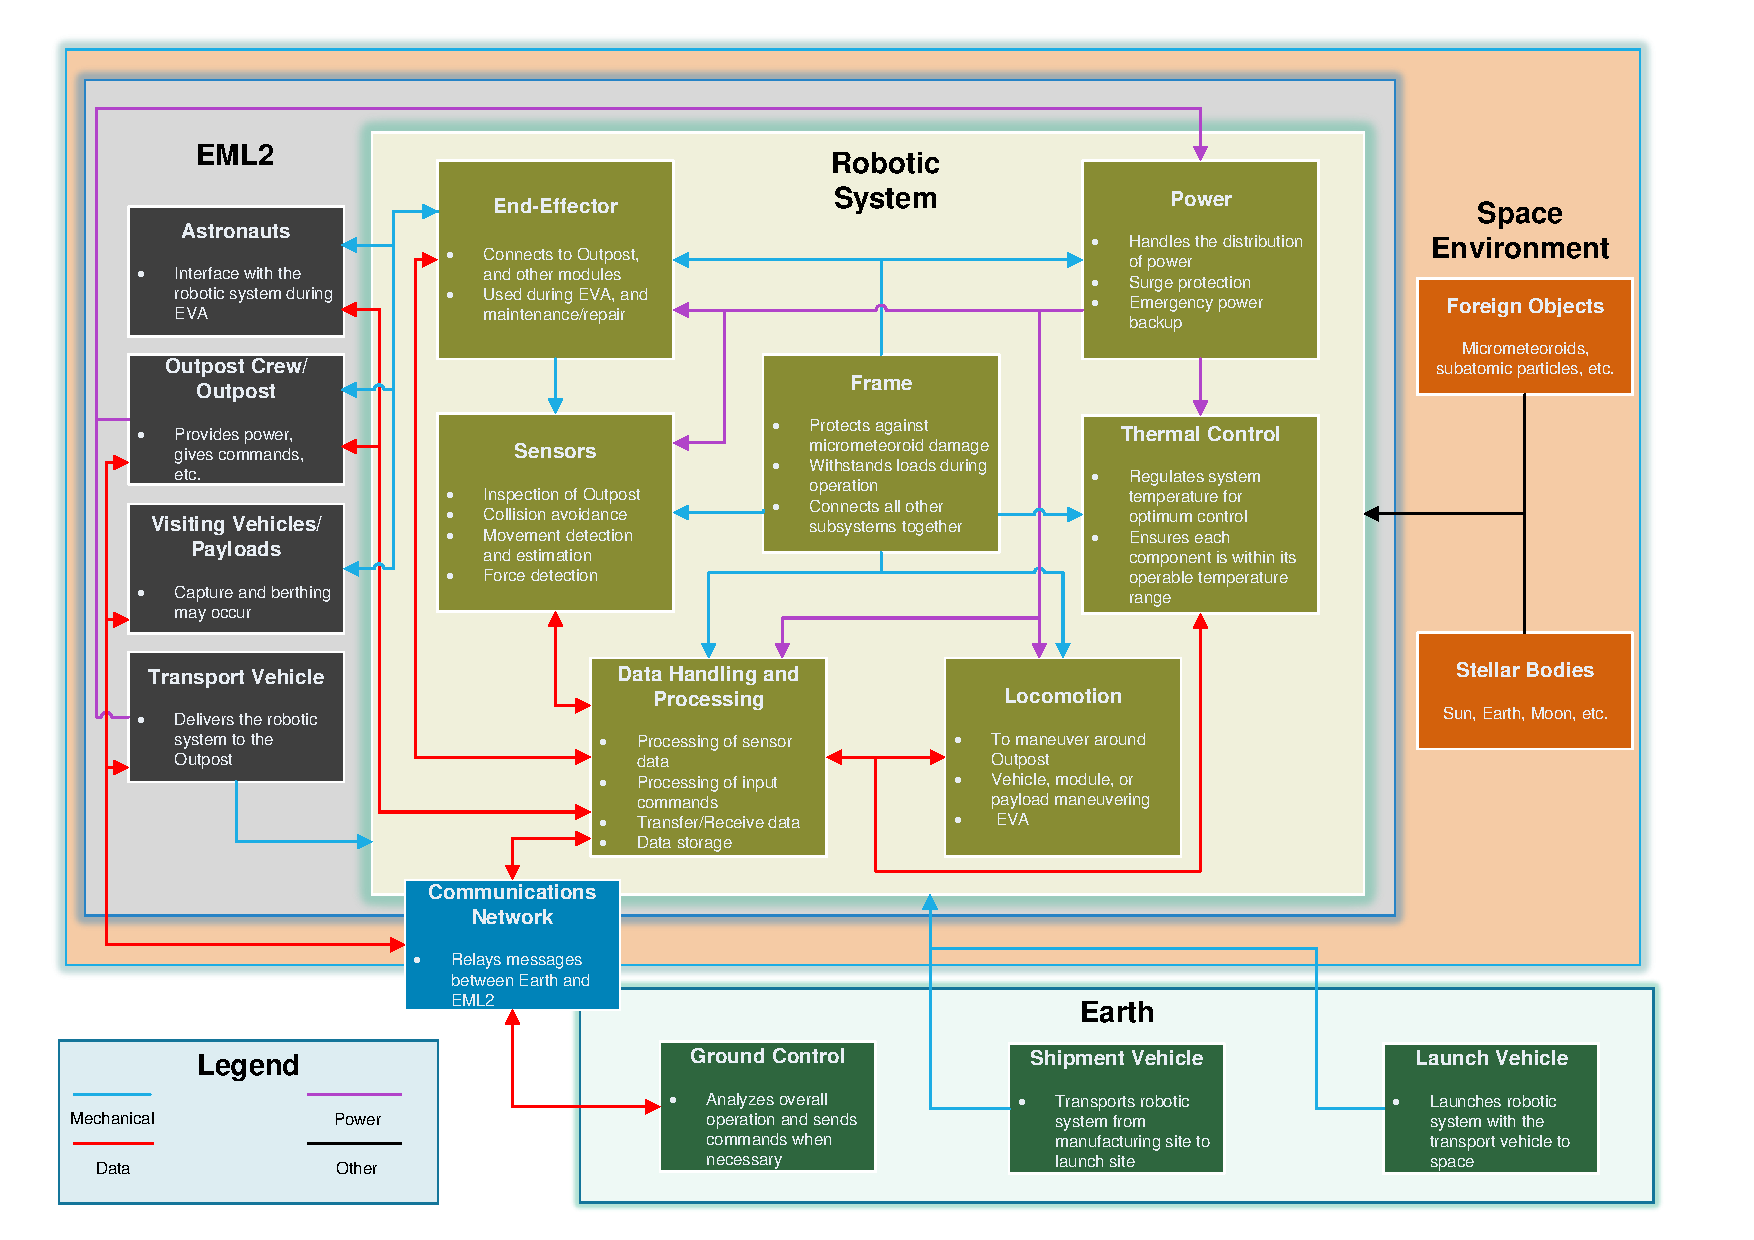
\includegraphics[height=0.9\textheight]{SBD}
\caption{System Block Diagram}
\label{fig:SBD}
\end{figure}
\end{landscape}
The complex number of different interfaces were categorized into general categories: mechanical, power, data, and other. In addition, double arrows indicate a two-sided relationship, whereas a single arrow is used to indicate a mainly one direction of interaction. Firstly, mechanical interfaces can be described as any sort of physical interfaces between two subsystems. For example, the end-effectors mechanically attach to the Outpost, astronauts during EVA, and provide a connection for many of the sensors. Secondly, power interfaces refer to the electrical power required to operate the robotic system. The power subsystem provides power to all the other internal subsystems (except the frame), and receives power from the Outpost and the transport vehicle. 

\vspace*{3pt}
Thirdly, data interfaces are very general, and refer to the sensor data, commands, and other communications being sent/received. In most cases, a combination of these different types of data is exchanged. Fourthly, an ``Other" interface occurs between the foreign objects and robotic system, which refers to the micrometeoroids, subatomic particles, and other debris that may physically interact with the robotic system. Moreover, the ``Other" interaction between stellar bodies and the robotic system refer to the emission of radiation, and the presence of microgravity.

\vspace*{3pt}
As there are a large amount of interfaces between the external subsystems themselves, it was deemed appropriate to omit these interfaces and focus on the internal-external interfaces. It is also important to note that the ``Communications Network" is a vast subsystem that starts on the Earth and up to and beyond the Outpost, hence it is situated in an overlapping position between the different block categories.

%--------------------------------------------------------------------------------------------------------------------------------------------------------------------------------
\section{System Hierarchy Diagram}
\label{sect:SHD}
The following diagram demonstrates the overall hierarchy of the robotic system:
\begin{figure}[H]
\label{fig:SHD}
\centering
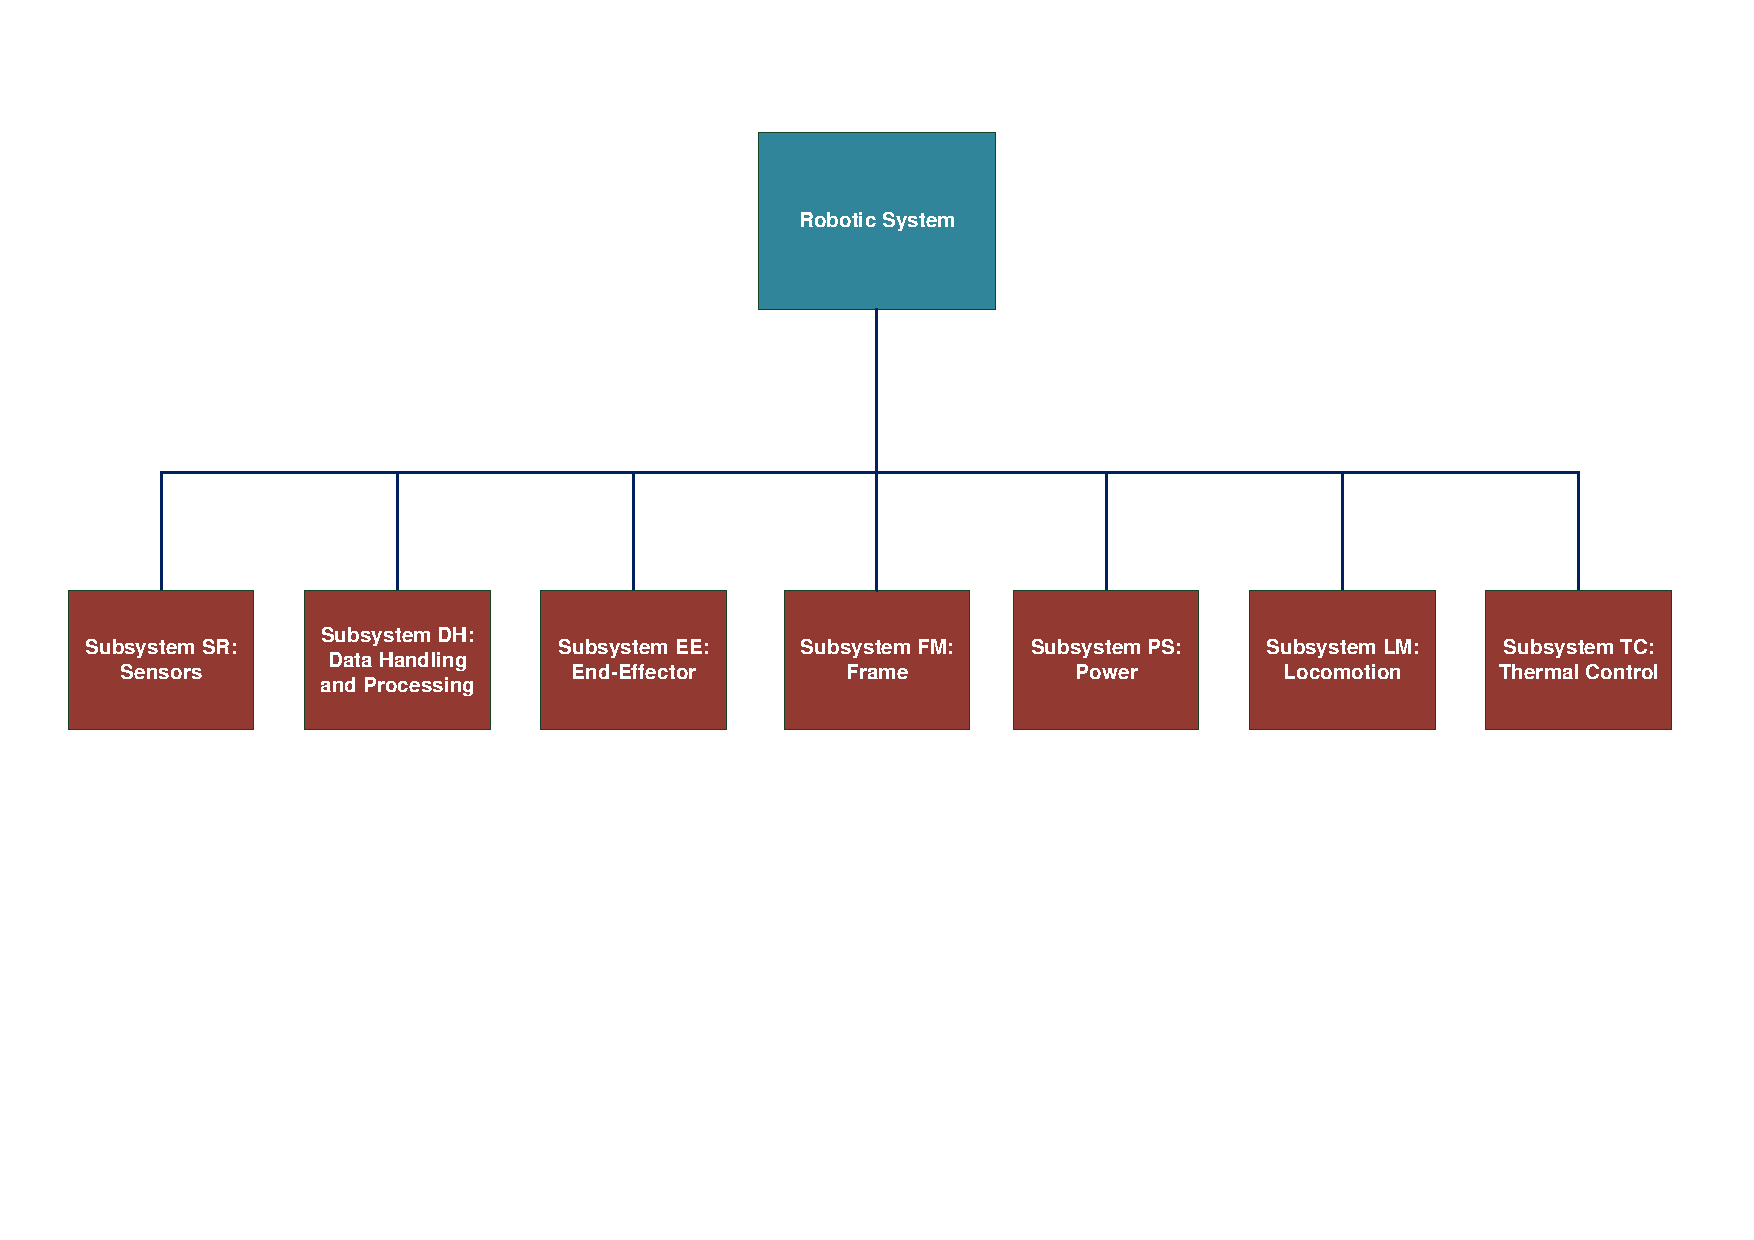
\includegraphics[width=0.9\textwidth]{SHD}
\caption{System Hierarchy Diagram}
\end{figure}

\section{Subsystem Requirements}
\label{sect:subsysreq}
In this section, the system requirements outlined in \Cref{sect:sysreq} are broken down in greater detail. Furthermore, these requirements are sub-categorized based on the internal subsystem that is primarily responsible. 

\subsection{Subsystem LM: Locomotion}
The locomotion subsystem is responsible for navigating around the Outpost, as well as moving the astronauts, modules, visiting vehicles and payloads to their desired destinations. The subsystem requirements for the locomotion subsystem are shown below.
\vspace{-5pt}
\begin{longtable}{P{2cm}P{13.75cm}}
\textbf{LM-F-01}	& The subsystem shall be able to be deployed from the transport vehicle. \textit{(Testing)}							\\
\textbf{LM-F-02}	& The subsystem shall be able to attach to the Outpost. \textit{(Simulation)}										\\
\textbf{LM-F-03}	& The subsystem shall be able to navigate Outpost modules. \textit{(Simulation)}										\\
\textbf{LM-F-04}	& The subsystem shall accept power from the power subsystem. \textit{(Testing)}										\\
\textbf{LM-F-05}	& The subsystem shall receive signals from the data handling subsystem. \textit{(Testing)}								\\
\end{longtable}
\vspace{-10pt}
\begin{longtable}{P{2cm}P{13.75cm}}
\textbf{LM-P-01}	& The subsystem shall cover TBD \% of the Outpost. \textit{(Simulation)}												\\
\textbf{LM-P-02}	& The subsystem shall move at TBD \si{\m\per\s} speed. \textit{(Simulation)}											\\
\textbf{LM-P-03}	& The subsystem shall operate for 10 years \cite{RFP}. \textit{(Analysis)}										\\
\end{longtable}
\vspace{-10pt}
\begin{longtable}{P{2cm}P{13.75cm}}
\textbf{LM-C-01}	& The subsystem shall weigh less than \SI{195}{\kg} (TBC) \cite{ERAjoint}. \textit{(Analysis)}							\\
\textbf{LM-C-02}	& The subsystem shall consume maximum TBD \si{\watt} of power. \textit{(Testing)}								\\
\textbf{LM-C-03}	& The subsystem shall be able to be transported from the manufacturing site to the launch site. \textit{(Analysis)}	\\
\end{longtable}
\vspace{-10pt}
\begin{longtable}{P{2cm}P{13.75cm}}
\textbf{LM-E-01}	& The system shall operate in a vacuum environment. \textit{(Testing)}													\\
\textbf{LM-E-02}	& The subsystem shall operate at temperature range of \SI{-70}{\degreeCelsius} to \SI{180}{\degreeCelsius} (TBC) \cite{NASAsysreq_Kumar}. \textit{(Testing)}										\\
\textbf{LM-E-03}	& The subsystem shall withstand vibrations sustained during transport to launch site. \textit{(Simulation)}		\\
\textbf{LM-E-04}	& The subsystem shall withstand vibrations sustained during launch. \textit{(Simulation)}						\\
\end{longtable}

\subsection{Subsystem DH: Data Handling and Processing}
The data handling and processing subsystem is responsible for performing necessary computations, collecting data from sensors, while sending and receiving data to different internal and external subsystems. The subsystem requirements for the data handling and processing subsystem are shown below.
\vspace{-5pt}
\begin{longtable}{P{2cm}P{13.75cm}}
\textbf{DH-F-01}	& The subsystem shall send transmissions to the Outpost. \textit{(Simulation)}										\\
\textbf{DH-F-02}	& The subsystem shall receive transmissions from the Outpost. \textit{(Simulation)}									\\
\textbf{DH-F-03}	& The subsystem shall receive transmissions from Ground Control. \textit{(Simulation)}								\\
\textbf{DH-F-04}	& The subsystem shall process these transmissions for computation. \textit{(Testing)}									\\
\textbf{DH-F-05}	& The subsystem shall process the data received from sensors. \textit{(Testing)}										\\
\textbf{DH-F-06}	& The subsystem shall accept power from the Power Subsystem. \textit{(Testing)}										\\
\end{longtable}
\vspace{-10pt}
\begin{longtable}{P{2cm}P{13.75cm}}
\textbf{DH-P-01}	& The subsystem shall send transmissions at (TBD) speed. \textit{(Testing)}											\\
\textbf{DH-P-02}	& The subsystem shall operate for 10 years \cite{RFP}. \textit{(Analysis)}										\\
\end{longtable}
\vspace{-10pt}
\begin{longtable}{P{2cm}P{13.75cm}}
\textbf{DH-C-01}	& The subsystem shall weigh less than TBD \si{\kg}. \textit{(Analysis)}													\\
\textbf{DH-C-02}	& The subsystem shall store minimum TBD \si{\giga\byte} of data. \textit{(Analysis)}									\\
\textbf{DH-C-03}	& The subsystem shall consume maximum TBD \si{\watt} of power. \textit{(Testing)}								\\
\textbf{DH-C-04}	& The subsystem shall be able to be transported from the manufacturing site to the launch site. \textit{(Analysis)}	\\
\end{longtable}
\vspace{-10pt}
\begin{longtable}{P{2cm}P{13.75cm}}
\textbf{DH-E-01}	& The system shall operate in a vacuum environment. \textit{(Testing)}													\\
\textbf{DH-E-02}	& The subsystem shall operate at temperature range of \SI{-20}{\degreeCelsius} to \SI{65}{\degreeCelsius} (TBC) \cite{NASAsysreq_Kumar}. \textit{(Testing)}										\\
\textbf{DH-E-03}	& The subsystem shall withstand vibrations sustained during transport to launch site. \textit{(Simulation)}		\\
\textbf{DH-E-04}	& The subsystem shall withstand vibrations sustained during launch. \textit{(Simulation)}						\\
\end{longtable}

\subsection{Subsystem TC: Thermal Control}
The thermal control subsystem is responsible for keeping track of temperatures of the other internal subsystems and ensuring they are operating within their acceptable temperature ranges. The subsystem requirements for the thermal control subsystem are shown below.

\vspace{-5pt}
\begin{longtable}{P{2cm}P{13.75cm}}
\textbf{TC-F-01}	& The subsystem shall track the temperature of all system components. \textit{(Testing)}								\\
\textbf{TC-F-02}	& The subsystem shall accept power from the power subsystem. \textit{(Testing)}										\\
\textbf{TC-F-03}	& The subsystem shall receive signal from the data handling subsystem. \textit{(Testing)}								\\
\end{longtable}
\vspace{-10pt}
\begin{longtable}{P{2cm}P{13.75cm}}
\textbf{TC-P-01}	& The subsystem shall maintain the temperature of each components at operational levels refer to table in \Cref{app:optemp} (TBC). \textit{(Testing)}							\\
\textbf{TC-P-02}	& The subsystem shall operate for 10 years \cite{RFP}. \textit{(Analysis)}										\\
\end{longtable}
\vspace{-10pt}
\begin{longtable}{P{2cm}P{13.75cm}}
\textbf{TC-C-01}	& The subsystem shall weigh less than TBD \si{\kg}. \textit{(Analysis)}													\\
\textbf{TC-C-02}	& The subsystem shall consume maximum TBD \si{\watt} of power. \textit{(Testing)}								\\
\textbf{TC-C-03}	& The subsystem shall be able to be transported from the manufacturing site to the launch site. \textit{(Analysis)}	\\
\end{longtable}
\vspace{-10pt}
\begin{longtable}{P{2cm}P{13.75cm}}
\textbf{TC-E-01}	& The system shall operate in a vacuum environment. \textit{(Testing)}													\\
\textbf{TC-E-02}	& The subsystem shall operate at temperature range of TBD. \textit{(Testing)}											\\
\textbf{TC-E-03}	& The subsystem shall withstand vibrations sustained during transport to launch site. \textit{(Simulation)}		\\
\textbf{TC-E-04}	& The subsystem shall withstand vibrations sustained during launch. \textit{(Simulation)}						\\
\end{longtable}

\subsection{Subsystem PS: Power Subsystem}
The power subsystem is responsible for distributing power to other subsystems and ensuring the other subsystems function properly. The subsystem requirements for the power subsystem are shown below.

\vspace{-5pt}
\begin{longtable}{P{2cm}P{13.75cm}}
\textbf{PS-F-01}	& The subsystem shall accept power from an external supply (Outpost or transport vehicle). \textit{(Testing \& Simulation)}																		\\
\textbf{PS-F-02}	& The subsystem shall supply all internal subsystems (except the frame) with power. \textit{(Testing)}			\\
\textbf{PS-F-03}	& The subsystem shall mitigate power surges. \textit{(Testing \& Simulation)}									\\
\end{longtable}
\vspace{-10pt}
\begin{longtable}{P{2cm}P{13.75cm}}
\textbf{PS-P-01}	& The subsystem shall provide power to the other subsystems without interruption. \textit{(Testing \& Simulation)}	\\
\textbf{PS-P-02}	& The subsystem shall operate for 10 years \cite{RFP}. \textit{(Analysis)}										\\
\end{longtable}
\vspace{-10pt}
\begin{longtable}{P{2cm}P{13.75cm}}
\textbf{PS-C-01}	& The subsystem shall weigh less than TBD \si{\kg}. \textit{(Analysis)}													\\
\textbf{PS-C-02}	& The average power shall be less than \SI{450}{\watt} \cite{RFP}. \textit{(Testing)}								\\
\textbf{PS-C-03}	& The peak power shall be less than \SI{600}{\watt} \cite{RFP}. \textit{(Testing)}										\\
\textbf{PS-C-04}	& The subsystem shall be able to be transported from the manufacturing site to the launch site. \textit{(Analysis)}	\\
\end{longtable}
\vspace{-10pt}
\begin{longtable}{P{2cm}P{13.75cm}}
\textbf{PS-E-01}	& The system shall operate in a vacuum environment. \textit{(Testing)}													\\
\textbf{PS-E-02}	& The subsystem shall operate at temperature range of TBD. \textit{(Testing)}											\\
\textbf{PS-E-03}	& The subsystem shall withstand vibrations sustained during transport to launch site. \textit{(Simulation)}		\\
\textbf{PS-E-04}	& The subsystem shall withstand vibrations sustained during launch. \textit{(Simulation)}						\\
\end{longtable}

\subsection{Subsystem EE: End Effector}
The end effector subsystem is responsible for interacting with the external subsystems situated around EML2, including the Outpost, astronauts, visiting vehicles and payloads. The subsystem requirements for the end effector subsystem are shown below.

\vspace{-5pt}
\begin{longtable}{P{2cm}P{13.75cm}}
\textbf{EE-F-01}	& The subsystem shall be able to attach to astronauts for EVA. \textit{(Simulation)}							\\
\textbf{EE-F-02}	& The subsystem shall be able to capture visiting vehicles and payloads.	\textit{(Simulation)}						\\
\textbf{EE-F-03}	& The subsystem shall be able to detach faulty components. \textit{(Simulation)}									\\
\textbf{EE-F-04}	& The subsystem shall accept power from the Power Subsystem. \textit{(Testing)}										\\
\textbf{EE-F-05}	& The subsystem shall receive signal from the Data Handling Subsystem. \textit{(Testing)}								\\
\textbf{EE-F-06}	& The subsystem shall connect to ancillary equipments. \textit{(Testing)}										\\
\textbf{EE-F-07}	& The subsystem shall store ancillary equipment. \textit{(Testing)}													\\
\textbf{EE-F-08}	& The subsystem shall provide lighting to the work area when necessary. \textit{(Testing)}								\\
\end{longtable}
\vspace{-10pt}
\begin{longtable}{P{2cm}P{13.75cm}}
\textbf{EE-P-01}	& The subsystem shall manipulate payloads of up to \SI{10000}{\kg} (TBC) \cite{RFP}. \textit{(Testing)}					\\
\textbf{EE-P-02}	& The subsystem shall apply holding or reaction forces of \SI{200}{\N} in any direction. \textit{(Testing)}			\\
\textbf{EE-P-03}	& The subsystem shall accommodate for \SI{0}{\m} to \SI{0.1}{\m} (TBC) of linear misalignment in axial direction \cite{NASAsysreq_Kumar}. \textit{(Testing \& Simulation)}						\\
\textbf{EE-P-04}	& The subsystem shall accommodate for $\pm$ \SI{0.1}{\m} (TBC) of linear misalignment in radial direction \cite{NASAsysreq_Kumar}. \textit{(Testing \& Simulation)}						\\
\textbf{EE-P-05}	& The subsystem shall accommodate for $\pm$ \SI{10}{\degree} (TBC) roll of angular misalignment \cite{NASAsysreq_Kumar}. \textit{(Testing \& Simulation)}									\\
\textbf{EE-P-06}	& The subsystem shall accommodate for $\pm$ \SI{15}{\degree} (TBC) pitch and yaw of angular misalignment \cite{NASAsysreq_Kumar}. \textit{(Testing \& Simulation)}									\\
\textbf{EE-P-07}	& The subsystem shall have active compliance range from \SI{20}{lbs} to \SI{300}{lbs} (TBC) \cite{NASAEE_Mishkin}.	\textit{(Testing)}													\\
\textbf{EE-P-08}	& The subsystem shall operate for 10 years \cite{RFP}. \textit{(Analysis)}										\\
\end{longtable}
\vspace{-10pt}
\begin{longtable}{P{2cm}P{13.75cm}}
\textbf{EE-C-01}	& The subsystem shall weigh less than TBD \si{\kg}. \textit{(Analysis)}													\\
\textbf{EE-C-02}	& The subsystem shall consume maximum TBD \si{\watt} of power. \textit{(Testing)}								\\
\textbf{EE-C-03}	& The subsystem shall be able to be transported from the manufacturing site to the launch site. \textit{(Analysis)}	\\
\end{longtable}
\vspace{-10pt}
\begin{longtable}{P{2cm}P{13.75cm}}
\textbf{EE-E-01}	& The system shall operate in a vacuum environment. \textit{(Testing)}													\\
\textbf{EE-E-02}	& The subsystem shall operate at temperature range of \SI{-70}{\degreeCelsius} to \SI{180}{\degreeCelsius} (TBC) \cite{NASAsysreq_Kumar}. \textit{(Testing)}										\\
\textbf{EE-E-03}	& The subsystem shall withstand vibrations sustained during transport to launch site. \textit{(Simulation)}		\\
\textbf{EE-E-04}	& The subsystem shall withstand vibrations sustained during launch. \textit{(Simulation)}						\\
\textbf{EE-E-05}	& The subsystem shall withstand collision with foreign objects traveling at TBD \si{\m\per\s}. \textit{(Testing \& Simulation)}														\\
\textbf{EE-E-06}	& The subsystem shall withstand electromagnetic radiation of \SI{1300}{\watt\per\square\m} (TBC) \cite{FAA_radiation}. \textit{(Simulation)}												\\
\textbf{EE-E-07}	& The subsystem shall withstand solar flares. \textit{(Simulation)}												\\
\textbf{EE-E-08}	& The subsystem shall withstand cosmic rays. \textit{(Simulation)}												\\
\end{longtable}

\subsection{Subsystem SR: Sensors}
The sensor subsystem is responsible for monitoring the space environment and the robotic system to detect any problems and help make mission critical decisions. The subsystem requirements for the sensors subsystem are shown below.

\vspace{-5pt}
\begin{longtable}{P{2cm}P{13.75cm}}
\textbf{SR-F-01}	& The subsystem shall provide supporting structure to the robotic system. \textit{(Analysis)}							\\
\textbf{SR-F-02}	& The subsystem shall shield the inner components from some environmental hazards (i.e. micrometeoroids, charged particles, etc). \textit{(Testing \& Simulation)}					\\
\end{longtable}
\vspace{-10pt}
\begin{longtable}{P{2cm}P{13.75cm}}
\textbf{SR-P-01}	& The subsystem shall sense proximity of TBD \si{\m}.	\textit{Simulation}										\\
\textbf{SR-P-02}	& The subsystem shall have maximum 1\% total mass loss due to outgassing. \textit{(Testing)} \cite{NASA_outgassing}			\\
\textbf{SR-P-03}	& The subsystem shall detect flaws ranges from \SI{0.2}{\milli\meter} to \SI{0.6}{\milli\meter} (TBC) \cite{NASAinspect_Hayati}. \textit{(Testing)}				\\
\textbf{SR-P-04}	& The subsystem shall operate for 10 years \cite{RFP}. \textit{(Analysis)}										\\
\end{longtable}
\vspace{-10pt}
\begin{longtable}{P{2cm}P{13.75cm}}
\textbf{SR-C-01}	& The subsystem shall weigh less than TBD \si{\kg}. \textit{(Analysis)}													\\
\textbf{SR-C-02}	& The subsystem shall consume maximum TBD \si{\watt} of power. \textit{(Testing)}								\\
\textbf{SR-C-03}	& The subsystem shall be able to be transported from the manufacturing site to the launch site. \textit{(Analysis)}	\\
\end{longtable}
\vspace{-10pt}
\begin{longtable}{P{2cm}P{13.75cm}}
\textbf{SR-E-01}	& The system shall operate in a vacuum environment. \textit{(Testing)}													\\
\textbf{SR-E-02}	& The subsystem shall operate at temperature range of \SI{-20}{\degreeCelsius} to \SI{65}{\degreeCelsius} (TBC) \cite{NASAsysreq_Kumar}. \textit{(Testing)}										\\
\textbf{SR-E-03}	& The subsystem shall withstand vibrations sustained during transport to launch site. \textit{(Simulation)}		\\
\textbf{SR-E-04}	& The subsystem shall withstand vibrations sustained during launch. \textit{(Simulation)}						\\
\textbf{SR-E-05}	& The subsystem shall withstand collision with foreign objects traveling at TBD \si{\m\per\s}. \textit{(Testing \& Simulation)}														\\
\textbf{SR-E-06}	& The subsystem shall withstand electromagnetic radiation of \SI{1300}{\watt\per\square\m} (TBC) \cite{FAA_radiation}. \textit{(Simulation)}												\\
\textbf{SR-E-07}	& The subsystem shall withstand solar flares. \textit{(Simulation)}												\\
\textbf{SR-E-08}	& The subsystem shall withstand cosmic rays. \textit{(Simulation)}												\\
\end{longtable}

\subsection{Subsystem FR: Frame}
The frame subsystem is responsible for providing structural support to the robotic system, and protect inner subsystems from some of the environmental hazards. The subsystem requirements for the frame subsystem are shown below.

\vspace{-5pt}
\begin{longtable}{P{2cm}P{13.75cm}}
\textbf{FR-F-01}	& The subsystem shall provide supporting structure to the robotic system. \textit{(Analysis)}							\\
\textbf{FR-F-02}	& The subsystem shall shield the inner components from some environmental hazards (i.e. micrometeoroids, charged particles, etc). \textit{(Testing \& Simulation)}					\\
\end{longtable}
\vspace{-10pt}
\begin{longtable}{P{2cm}P{13.75cm}}
\textbf{FR-P-01}	& The subsystem shall have minimum TBD \si{\K\per\watt} of thermal resistance. \textit{(Testing)}						\\
\textbf{FR-P-02}	& The subsystem shall have minimum 1.1 yield safety factor (TBC) \cite{NASAsysreq_Kumar}. \textit{(Analysis)}						\\
\textbf{FR-P-03}	& The subsystem shall have minimum 1.5 ultimate safety factor (TBC) \cite{NASAsysreq_Kumar}. \textit{(Analysis)}				\\
\textbf{FR-P-04}	& The subsystem shall have maximum 1\% total mass loss due to outgassing \cite{NASA_outgassing}. \textit{(Testing)}			\\
\textbf{FR-P-05}	& The subsystem shall withstand TBD \si{N} of force. \textit{(Testing)}													\\
\textbf{FR-P-06}	& The subsystem shall withstand TBD \si{\N\m} of torque. \textit{(Testing)}											\\
\textbf{FR-P-07}	& The subsystem shall operate for 10 years \cite{RFP}. \textit{(Analysis)}										\\
\end{longtable}
\vspace{-10pt}
\begin{longtable}{P{2cm}P{13.75cm}}
\textbf{FR-C-01}	& The subsystem shall weigh less than TBD \si{\kg}. \textit{(Analysis)}													\\
\textbf{FR-C-02}	& The dimensions of the frame components shall be less than (TBD). \textit{(Analysis)}									\\
\textbf{FR-C-03}	& The subsystem shall be able to be transported from the manufacturing site to the launch site. \textit{(Analysis)}	\\
\end{longtable}
\vspace{-10pt}
\begin{longtable}{P{2cm}P{13.75cm}}
\textbf{FR-E-01}	& The system shall operate in a vacuum environment. \textit{(Testing)}													\\
\textbf{FR-E-02}	& The subsystem shall withstand vibrations sustained during transport to launch site. \textit{(Simulation)}		\\
\textbf{FR-E-03}	& The subsystem shall withstand vibrations sustained during launch. \textit{(Simulation)}						\\
\textbf{FR-E-04}	& The subsystem shall withstand collision with foreign objects traveling at TBD \si{\m\per\s}. \textit{(Testing \& Simulation)}														\\
\textbf{FR-E-05}	& The subsystem shall withstand electromagnetic radiation of \SI{1300}{\watt\per\square\m} (TBC) \cite{FAA_radiation}. \textit{(Simulation)}												\\
\textbf{FR-E-06}	& The subsystem shall withstand solar flares. \textit{(Simulation)}												\\
\textbf{FR-E-07}	& The subsystem shall withstand cosmic rays. \textit{(Simulation)}												\\
\end{longtable}
\captionsetup[table]{list=yes}
\setcounter{table}{0}
%--------------------------------------------------------------------------------------------------------------------------------------------------------------------------------
\newpage
\section{Drivers}
\label{sect:drivers}
The following five requirements are identified as the key design drivers, which will heavily influence the outcome of system design.
\subsubsection*{S-F-04: Shall perform regular inspection of the Outpost}
The requirement that the system be able to perform regular inspection of the Outpost influences the locomotion and power subsystem designs. An actuator with sufficient torque to allow the system move around the Outpost and a power subsystem which provides sufficient power to the actuators will be required. In addition, the sensor subsystems have to be accurate enough to inspect the condition of the Outpost, while the data handling subsystems should be able to process all the data collected in order to give commands on maintenance and repair operations.
\subsubsection*{S-P-05: Shall be able to cover TBD \% of Outpost}
The requirement that the system has to be able to cover TBD \% of Outpost influences the locomotion and end-effector design, as well as the positioning of sensors to ensure that the sensor subsystem is able to analyze the Outpost in detail. In addition, design decisions regarding how the system is able to reach to the ends of the Outpost would also have to be decided. Naturally, the frame subsystem is affected as the design of the robotic system changes.
\subsubsection*{S-C-01: Shall have a mass of less than 450 kg}
The constraint on mass affects the design of all subsystems. This driver influences the materials chosen for the frame, and end-effector subsystem. Additionally, the method of power supply, the types and amounts of sensors used on the robotic system is affected, as well as the hardware of the data handling, and thermal control subsystem. All these design decisions need to be made to fulfill the overall mass requirement. Moreover, the weight of the whole system will also have an influence on the method of shipment.
\subsubsection*{S-C-04: Average power usage of less than 450 W}
The power constraint influences all electrical components of the robotic system. It affects the types of sensors selected, the method of power supply and power backup, as well as the hardware choice of the data handling and processing, and thermal control subsystems. In order to complete all the operations within the power constraint, the mobility method of locomotion subsystem and electrical hardware of the data handling subsystem will also be influenced.
\subsubsection*{S-E-08: Shall withstand strikes by foreign objects traveling at TBD m/s}
This environmental requirement influences the material used for the frame and the thickness of the frame, and will therefore influence the structure design of the whole robotic system, while limiting the amount of mass allocated to other subsystems. In addition, this requirement affects the sensors selected, restricts the material of the camera lens and materials of other components on the robotic system that interfaces with the external environment. Furthermore, precautions must be taken to ensure that the end-effector subsystem can operate in such an environment.
%--------------------------------------------------------------------------------------------------------------------------------------------------------------------------------
\section{Trade-offs}
\label{sect:tradeoffs}
In this section, the major trade-offs in the design of the system will be discussed within three broad categories: mechanical, electrical and control/software. The text colors in the following tables correspond to desirability, with red being least , green being most desirable, and yellow being moderately desirable.
\subsection{Mechanical Trade-offs}
\subsubsection{Level of Autonomy}
The level of autonomy will determine how the operations should be planed and carried out, and will largely influence the design of data handling and control systems. Therefore, it should be discussed here as one of the major trade-offs. Three levels of autonomy are considered and compared, which are listed below and compared in \Cref{table:auto}. A limited-autonomous system requires Requires manual operations by the Outpost crew to complete all tasks, a semi-autonomous system shall be able to conduct basic tasks automatically, like change positions, but will require manual control by Outpost crew to complete more complex tasks while a fully-autonomous system shall be able to complete both all tasks without human intervention. 
\begin{table}[H]
\caption{Trade Study for Level of Autonomy}
\begin{tabular}{|P{2.5cm}|P{4.1cm}|P{4.1cm}|P{4.0cm}|}
\hline
	&	\textbf{Limited Autonomous}	&	\textbf{Semi Autonomous}	&	\textbf{Fully Autonomous}	\\\hhline{|=|=|=|=|}
\textbf{System Complexity}	&	\textcolor{OliveGreen}{Easy to develop\newline Rich technological heritage}	&	\textcolor{orange}{Existing similar systems\newline Need software development for the specific operations}	&	\textcolor{red}{Technology is hard to achieve\newline Full software development needed}	\\\hline
\textbf{System Reliability}	&	\textcolor{red}{Operation is fully monitored, but human errors may occur}	&	\textcolor{orange}{Simple tasks may be affected by software and component malfunctions\newline Complex tasks may be affected by human errors}	&	\textcolor{OliveGreen}{Operation could be under software and component malfunctions\newline Human error is avoided.}	\\\hline
\textbf{Operation Duration}	&	\textcolor{red}{Requires control from the Outpost crew or Ground Control\newline Communication delays will extend the operation duration, average delay is between seconds to up to 20 minutes \cite{NASAcomm}}	&	\textcolor{OliveGreen}{Short for simple tasks}\newline\textcolor{orange}{Longer duration for more complex tasks, assistance from Outpost crew is required}	&	\textcolor{OliveGreen}{ No human input required\newline Can operate continuously}	\\\hline
\textbf{Operation Accuracy \& Deviation from plans}	&	\textcolor{OliveGreen}{Accuracy is high due to manual control}\newline\textcolor{orange}{May be affected by human errors\newline Deviation from plans is limited by human control}	&	\textcolor{OliveGreen}{Accuracy will not be limited by computational resources for simple tasks\newline Human errors and robotic malfunctions are limited due to the cooperation between human and system\newline Deviation from plans limited}	&	\textcolor{orange}{Accuracy level limited by computational resources\newline Deviations may happen due to software or component malfunction\cite{NASAauto}}	\\\hline
\end{tabular}
\label{table:auto}
\end{table}

While a fully autonomous system would be ideal for space exploration because it would have high capabilities and efficiency, there are still technical, computational, safety and managerial challenges to overcome before achieving full autonomy. Therefore, taking current technology availability into consideration, a semi-autonomous system has been selected for this robotic system. This will allow the system to perform with relatively lower risk and higher efficiency.

\subsubsection{Passive vs. Active Thermal Control}
Thermal regulation systems are required in the system to ensure that temperatures of the system’s parts are within the operating ranges. There are two main types of such systems, Active Thermal Control System (ATCS) and Passive Thermal Control System (PTCS). 

ATCS makes use of various heating and cooling tools, such as electric heaters, fluid loops and thermoelectric coolers to control the temperature within the system while PTCS makes use of insulation to reduce heat transfer and surface coatings which modify the thermal or optical properties of the surface. These two systems are compared in \Cref{table:thermal}.
\begin{table}[H]
\caption{Trade Study for Type of Thermal Control System}
\begin{tabular}{|P{2.5cm}|P{6.35cm}|P{6.35cm}|}
\hline
	&	\textbf{ATCS}	&	\textbf{PTCS}	\\\hhline{|=|=|=|}
\textbf{System Complexity}	&	\textcolor{red}{Complex control system needed to respond rapidly to temperature fluctuations}	&	\textcolor{OliveGreen}{Only mechanical parts are added\newline Only increases mass, not complexity}	\\\hline
\textbf{System Reliability}	&	\textcolor{OliveGreen}{Outpost crew can manually control the temperature in case of breakdown in control system}\newline\textcolor{orange}{In case of breakdown of the heating and/or cooling elements, only solution is to repair them}	&	\textcolor{red}{Damage will result in loss of ability to maintain other subsystems at their operational temperature ranges}	\\\hline
\textbf{System Efficiency}	&	\textcolor{OliveGreen}{System can be on Standby mode when temperatures are within operating ranges\newline Only needs to be switched on when temperature is near the limits of operation; Saves power and does its job}	&	\textcolor{OliveGreen}{System can reduce heat transfer without using any power; Very efficient when there is alternating high and low temperatures}\newline\textcolor{orange}{System is unable to regulate temperatures when there is prolonged periods of extreme temperatures}	\\\hline
\end{tabular}
\label{table:thermal}
\end{table}
\newpage
It is decided that our robotic system will have a combination of Active and Passive Thermal Control Systems. The main system will be the passive system to slow down the rate of heat transfer between internal components and the exterior environment. The active system will activate when there is excessive heat transfer that the passive system is unable to manage, or when there is damage to the passive system. This allows us to achieve the advantages of power saving and single-fault tolerance in the thermal control system, but we would have to accept the consequence of increasing the mass of the system and designing a more complex control architecture for the active system.

\subsection{Electrical Trade-offs}
\subsubsection{Need for an Independent Power Generation System}
In order to provide the system with an independent power supply, power generators, such as solar panels, will need to be included as part of the system. This would significantly increase the complexity and weight of the system. In addition, as the system is not expected to spend a prolonged period of time detached from the Outpost, it is decided that the system will not have its own power generation unit and would instead be powered entirely by the Outpost. However, the system will have a power storage system which will be charged while the system is connected to the Outpost and can be used when there is a loss in connection between the Outpost and the system.

\subsection{Control/Software Trade-offs}
\subsubsection{Need for Direct Communications with Earth-based Ground Control}
Having a direct communications link with Ground Control would allow Ground Control to control the system in cases of a breakdown in connection between Outpost and system. However, in order to create such a link would require the addition of a communications subsystem in the robotic system and the setup of a communications network to handle such communications. The power required for the operation of a communications system is relatively low at about \SI{15}{\watt} to \SI{30}{\watt}\cite{Marscomm} and the mass is low compared to the maximum mass constraints of the robotics system. In addition, although there will be a time lag in command signals, it is not extremely long to cause impracticalities in conducting Earth-based teleoperation\cite{roboserve}. Hence, it has been decided that our system will contain a communications subsystem to communicate with Ground Control through various communications networks already in place. This will allow for emergency operation of the system from Earth in cases of a loss of communication between the Outpost and system.
%--------------------------------------------------------------------------------------------------------------------------------------------------------------------------------
\section{Conclusion}
\label{sect:conclusion}
In this report, the top-level requirements of a robotic system for the development and maintenance of a lunar Outpost were discussed. This was followed by an illustration of the seven robotic subsystems  frame, power, end-effector, data handling and processing, thermal control, sensors, and locomotion) in a System Block Diagram, showing the various interfaces between the robotic subsystems and external subsystems. Next, a System Hierarchy Diagram was displayed, followed by a detailed list of the numerous subsystem requirements. Additionally, the key drivers were identified, including weight, power, payload handling, inspection performance, and durability against foreign objects. Finally, the major mechanical, electrical, and control/software trade-offs were discussed. It was decided that a semi-autonomous system, a mix of PTCS and ATCS, a backup Ground Control communications, and a battery backup shall be used.
%--------------------------------------------------------------------------------------------------------------------------------------------------------------------------------
\newpage
\bibliographystyle{unsrt}
\bibliography{reportbib}

\newpage
\appendix
\section{Temperature Range of Components}
\label{app:optemp}
\begin{table}[H]
\caption[Operational and Survival Temperature Ranges of various Components]{Operational and Survival Temperature Ranges of various Components \cite{NASAsysreq_Kumar}}
\centering
\begin{tabular}{|l|l|l|}
\hline
\textbf{Component}	&	\textbf{Operational (\si{\degreeCelsius})}	&	\textbf{Survival (\si{\degreeCelsius})}\\\hhline{|=|=|=|}
\textbf{Gears \& Bearings}		&	-25 to 135	&	-50 to 155	\\\hline
\textbf{Motor Windings}			&	-25 to 180	&	-50 to 200	\\\hline
\textbf{Brakes}					&	-25 to 99	&	-50 to 120	\\\hline
\textbf{Cables \& Connectors}	&	-70 to 135	&	-90 to 155	\\\hline
\textbf{Electronics}			&	-20 to 65	&	-50 to 85	\\\hline
\end{tabular}
\end{table}
\newpage
\section{Data from External Documents}
\begin{figure}[H]
\centering
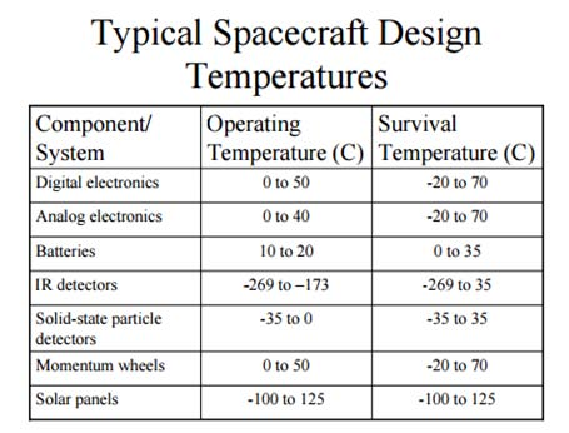
\includegraphics[scale=1]{Apppic/designtemp}
\caption[Typical Spacecraft Design Temperatures]{Typical Spacecraft Design Temperatures \cite{spacedesigntemp}}
\end{figure}
\begin{figure}[H]
\centering
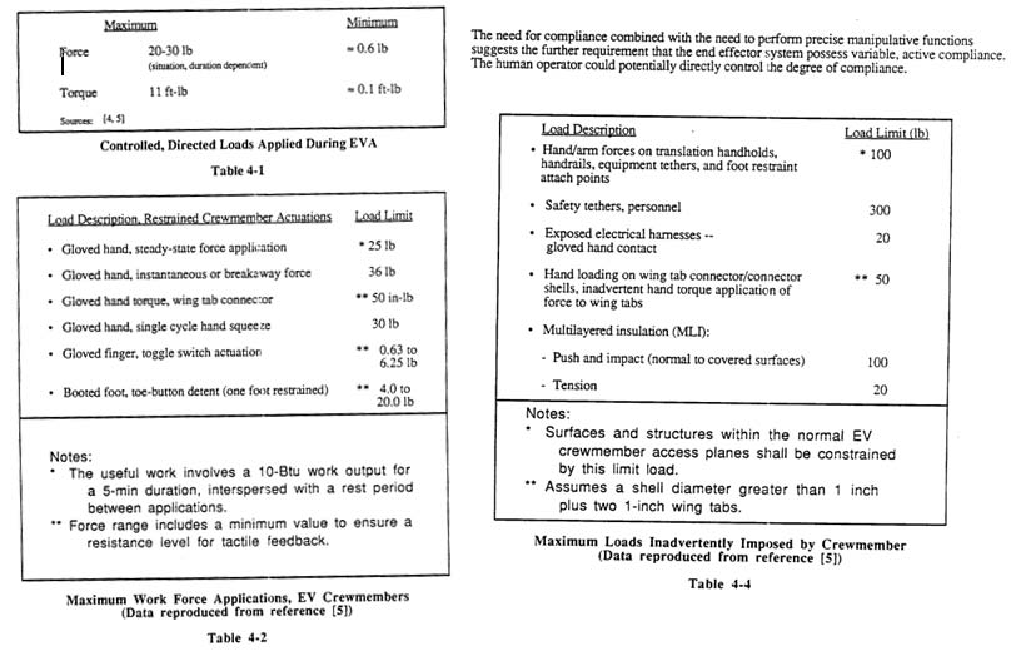
\includegraphics[scale=1]{Apppic/eeloads}
\caption[End Effector Load Limits]{End Effector Load Limits \cite{NASAEE_Mishkin}}
\end{figure}
\begin{figure}[H]
\centering
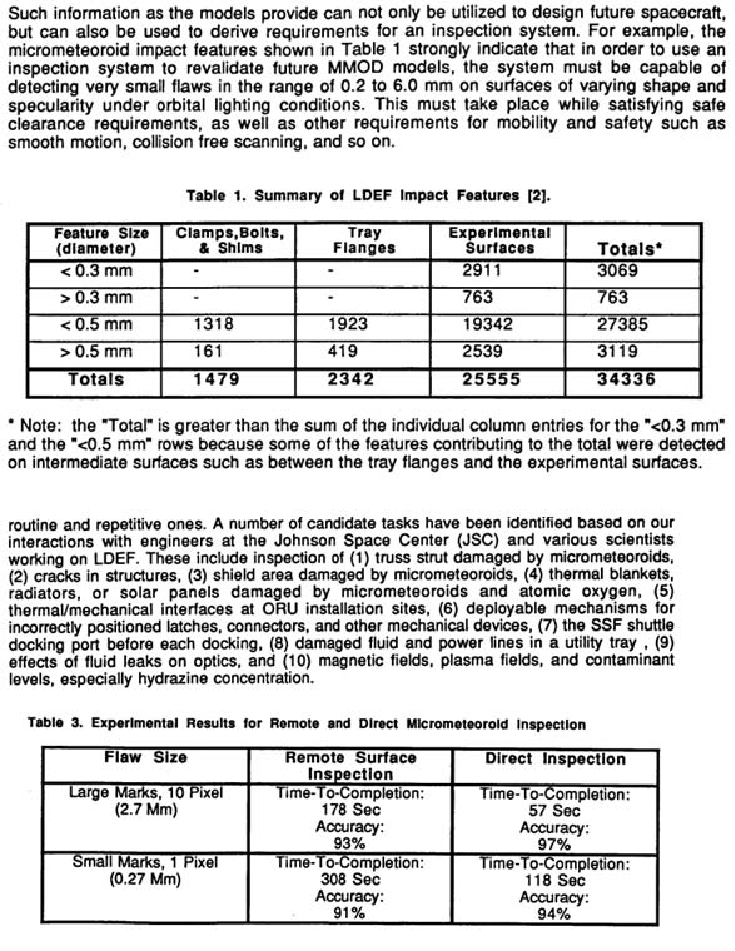
\includegraphics[scale=1]{Apppic/inspect}
\caption[Requirements for Inspection Systems]{Requirements for Inspection Systems \cite{NASAinspect_Hayati}}
\end{figure}

\end{document}
